\chapter{Arhitektura i dizajn sustava}
		
		Korištena arhitektura se može podijeliti na tri podsustava:
		    \begin{packed_item}
		        \item Web poslužitelj
    		    \item Web aplikacija
    		    \item Baza podataka
		    \end{packed_item}
		    
	    \underline{\textit{Web preglednik}} program je koji omogućuje pregled web-stranica i multimedijalnih sadržaja vezanih uz njih. Svaki internetski preglednik ima i ulogu prevoditelja, odnosno on interpretira kod kojim je stranica napisana i tako realizira grafičko sučelje i neke jednostavnije funkcionalnosti. Korisnik putem web preglednika šalje zahtjeve web poslužitelju.
	    
	    \underline{\textit{Web poslužitelj}} centralna je komponenta za rad web aplikacije. Njegova je glavna zadaća komunikacija klijenta s aplikacijom. Komunikacija se odvija preko HTTP (engl. \textit{Hyper Text Transfer Protocol}) protokola koji se koristi u prijenosu informacija na webu. Poslužitelj je onaj koji pokreće web aplikaciju, zaprima korisničke zahtjeve i prosljeđuje ih aplikaciji na obradu. Web poslužitelj koji smo odabrali za našu web aplikaciju je DigitalOcean. Na njega smo postavili naše \textit{frontend} i \textit{backend} komponente, a kao poslužitelj baze podataka odlučili smo koristiti Render.

	    Korisnik koristi \underline{\textit{web aplikaciju}} za obrađivanje željenih zahtijeva. Web aplikacija obrađuje zahtjev te ovisno o zahtjevu, pristupa bazi podataka nakon čega preko poslužitelja vraća korisniku odgovor u obliku HTML dokumenta vidljivog u web pregledniku.
		
		Programski jezik kojeg smo odabrali za izradu naše web aplikacije je Python zajedno s Flask radnim okvirom te programski jezik TypeScript s React radnim okvirom u sklopu kojeg smo koristili CSS radni okvir Bootstrap. Odabrano razvojno okruženje je Microsoft Visual Studio. Arhitektura sustava temeljit će se na MVC (Model-View-Controller) konceptu. MVC koncept podržan je od strane Flask radnog okvira i kao takav ima gotove predloške koji nam olakšavaju razvoj razvoj web aplikacije.
		
        Karakteristika MVC koncepta je nezavisan razvoj pojedinih dijelova aplikacije što za posljedicu ima jednostavnije ispitivanje kao i jednostavno razvijanje i dodavanje novih svojstava u sustav.
        MVC koncept sastoji se od:
        \begin{packed_item}
            \item \textbf{Model} – središnja komponenta sustava. Predstavlja dinamičke strukture podataka, neovisno o korisničkom sučelju. Izravno upravlja podacima, logikom i pravilima aplikacije te prima ulazne podatke od Controllera
            \item \textbf{View} – bilo kakav prikaz podataka, poput grafa. Mogući su različiti prikazi iste informacije poput grafičkog ili tabličnog prikaza podataka.
            \item \textbf{Controller} – prima ulaze i prilagođava ih za prosljeđivanje Modelu ili Viewu. Upravlja korisničkim zahtjevima i temeljem njih izvodi daljnju interakciju s ostalim elementima sustava.
        \end{packed_item}

		\pagebreak	
		\section{Baza podataka}
			
			Za potrebe našeg sustava koristit ćemo relacijsku bazu podataka koja svojom strukturom olakšava modeliranje stvarnog svijeta. Gradivna jedinka baze je relacija, odnosno tablica koja je definirana svojim imenom i skupom atributa. Zadaća baze podataka je brza i jednostavna pohrana, izmjena i dohvat podataka za daljnju obradu. Baza podataka ove aplikacije sastoji se od sljedećih entiteta:
			\begin{packed_item}
			    \item User
                \item Cartographer
                \item Player
                \item Admin
                \item Card
                \item Inventory
                \item Fight
                \item Challenge
			\end{packed_item}


		
			\subsection{Opis tablica}
			

				\textbf{User}   Ovaj entitet sadržava sve važne informacije o korisniku aplikacije, ali je apstraktan. Sadrži atribute: userID, username, name, email, profilePhoto, password, confirmed. Ovaj entitet je povezan s entitetima Player i Cartographer koji su specijalizacije entiteta User.
				
				
				\begin{longtblr}[
					label=none,
					entry=none
					]{
						width = \textwidth,
						colspec={|X[6,l]|X[6, l]|X[20, l]|}, 
						rowhead = 1,
					} %definicija širine tablice, širine stupaca, poravnanje i broja redaka naslova tablice
					\hline \multicolumn{3}{|c|}{\textbf{User}}	& \textbf{Type} & \textbf{Description}\\ \hline[3pt]
					\SetCell{LightGreen}userID & INT & jedinstveni identifikator korisnika\\ \hline
					username & VARCHAR & korisničko ime\\ \hline 
					name & VARCHAR & ime i prezime korisnika\\ \hline 
					email & VARCHAR	& email korisnika\\ \hline
					profilePhoto & VARCHAR & fotografija korisnika\\ \hline
					password & VARCHAR & lozinka korisnika\\ \hline
					confirmed & BOOLEAN & je li korisnik potvrđen putem emaila\\ \hline 
				\end{longtblr}
				
				
				\textbf{Cartographer}   Ovaj entitet sadržava sve važne informacije o korisniku aplikacije koji je kartograf. Sadrži atribute: userID, IBAN, document i verified. Ovaj entitet je specijalizacija entiteta User te je u vezi s entitetom Card preko atributa cartographerID.
				
				
				\begin{longtblr}[
					label=none,
					entry=none
					]{
						width = \textwidth,
						colspec={|X[6,l]|X[6, l]|X[20, l]|}, 
						rowhead = 1,
					} %definicija širine tablice, širine stupaca, poravnanje i broja redaka naslova tablice
					\hline \multicolumn{3}{|c|}{\textbf{Cartographer}}	& \textbf{Type} & \textbf{Description}\\ \hline[3pt]
					\SetCell{LightGreen}userID & INT & \SetCell{LightBlue}jedinstveni identifikator korisnika (user.userID)\\ \hline
					IBAN & VARCHAR & IBAN kartografa\\ \hline 
					document & VARCHAR & fotografija osobne iskaznice kartografa\\ \hline 
					verified & BOOLEAN	& je li administrator odobrio kartografa\\ \hline
				\end{longtblr}
				
			
			\textbf{Player}   Ovaj entitet sadržava sve važne informacije o korisniku aplikacije koji je igrač. Sadrži atribute: userID,  advanced, eloScore, banned i playerLocation. Ovaj entitet je specijalizacija entiteta User te je u vezi \textit{One-to-Many} s entitetom Inventory preko atributa userID te je u vezi \textit{One-to-Many} s entitetom Card preko atributa authorUserID. Također je u vezi \textit{One-to-Many} s entitetom Challenge preko atributa challengerUserID, tj. victimUserID kao što je i u \textit{One-to-Many} vezi s entiteom Fight preko atributa player1UserID, tj. player2UserID.
				
				
				\begin{longtblr}[
					label=none,
					entry=none
					]{
						width = \textwidth,
						colspec={|X[6,l]|X[6, l]|X[20, l]|}, 
						rowhead = 1,
					} %definicija širine tablice, širine stupaca, poravnanje i broja redaka naslova tablice
					\hline \multicolumn{3}{|c|}{\textbf{Player}}	& \textbf{Type} & \textbf{Description}\\ \hline[3pt]
					\SetCell{LightGreen}userID & INT & \SetCell{LightBlue}jedinstveni identifikator korisnika (user.userID)\\ \hline
					advanced	& BOOLEAN & razina ovlasti igrača može biti ordinary ili advanced\\ \hline 
					eloScore & INT & ELO score igrača\\ \hline 
					banned & BOOLEAN	& je li igrač isključen iz igre\\ \hline
					playerLocation & VARCHAR & aktivna lokacija korisnika\\ \hline
					signedIn & BOOLEAN & je li korisnik prijavljen u sustav\\ \hline
				\end{longtblr}
			\pagebreak
			
			\textbf{Admin}   Ovaj entitet sadržava sve važne informacije o adminu. Sadrži atribute: adminID, username, name, email, password.
				
				
				\begin{longtblr}[
					label=none,
					entry=none
					]{
						width = \textwidth,
						colspec={|X[6,l]|X[6, l]|X[20, l]|}, 
						rowhead = 1,
					} %definicija širine tablice, širine stupaca, poravnanje i broja redaka naslova tablice
					\hline \multicolumn{3}{|c|}{\textbf{Admin}}	& \textbf{Type} & \textbf{Description}\\ \hline[3pt]
					\SetCell{LightGreen}adminID & INT & jedinstveni identifikator admina\\ \hline
					username	& VARCHAR & korisničko ime\\ \hline 
					name & VARCHAR & ime i prezime admina\\ \hline 
					email & VARCHAR	& email admina\\ \hline
					password & VARCHAR & lozinka admina\\ \hline
				\end{longtblr}
				
				
			\textbf{Card}   Ovaj entitet sadržava sve važne informacije o kartici. Sadrži atribute: cardID, cardLocation, locationPhoto, title, description, cardStatus, authorUserID, cartographerID. Ovaj entitet je u vezi \textit{One-to-Many} s entitetom Inventory preko atributa cardID te je u \textit{One-to-Many} vezi s entitetom Fight preko atributa cardIDxy gdje je x element {1, 2} i y je element {1, 2, 3}. Card je također u \textit{One-to-One} vezi s entitetom Player preko atributa authorUserID te je u \textit{One-to-One} vezi s entitetom Cartographer preko atributa authorUserID.
				
				
				\begin{longtblr}[
					label=none,
					entry=none
					]{
						width = \textwidth,
						colspec={|X[12,l]|X[8, l]|X[20, l]|}, 
						rowhead = 1,
					} %definicija širine tablice, širine stupaca, poravnanje i broja redaka naslova tablice
					\hline \multicolumn{3}{|c|}{\textbf{Card}}	& \textbf{Type} & \textbf{Description}\\ \hline[3pt]
					\SetCell{LightGreen}cardID & INT & šifra kartice\\ \hline
					cardLocation & VARCHAR & lokacija kartice\\ \hline 
					locationPhoto & VARCHAR & fotografija kartice\\ \hline 
					title & VARCHAR	& naziv kartice\\ \hline
					description & VARCHAR & opis kartice\\ \hline
					cardStatus & ENUM & status kartice može biti: submitted, unclaimed, claimed, verified\\ \hline
					\SetCell{LightBlue}authorUserID & INT & koji igrač je predložio dodavanje nove kartice u igru (user.userID)\\ \hline 
					\SetCell{LightBlue}cartographerID & INT & koji kartograf je odobrio zahtjev za izradu nove kartice (user.userID)\\ \hline
				\end{longtblr}
			\pagebreak
				
			\textbf{Inventory}   Ovaj entitet sadržava sve važne informacije o karticama koje pojedini igrači posjeduju. Sadrži atribute: userID, cardID i strength. Ovaj entitet je u \textit{Many-to-One} vezi s entitetom Player preko atributa userID te u \textit{Many-to-One} vezi s entitetom Card preko atributa cardID.
				
				
				\begin{longtblr}[
					label=none,
					entry=none
					]{
						width = \textwidth,
						colspec={|X[6,l]|X[6, l]|X[20, l]|}, 
						rowhead = 1,
					} %definicija širine tablice, širine stupaca, poravnanje i broja redaka naslova tablice
					\hline \multicolumn{3}{|c|}{\textbf{Inventory}}	& \textbf{Type} & \textbf{Description}\\ \hline[3pt]
					\SetCell{LightGreen}userID & INT & \SetCell{LightBlue}identifikacijski broj korisnika koji posjeduje karticu (user.userID)\\ \hline
					\SetCell{LightGreen}cardID	& INT & \SetCell{LightBlue}šifra kartice\\ \hline 
					strength & INT & jačina kartice\\ \hline
				\end{longtblr}
				
				
			\textbf{Fight}   Ovaj entitet sadržava sve važne informacije o borbi između dva igrača. Sadrži atribute: fightID, player1UserID, player2UserID, cardID11, cardID12, cardID13, cardID21, cardID22, cardID23, points1, points2, fightTimestamp, challengeID. Ovaj entitet je u \textit{One-to-One} vezi s entitetom Challenge preko atributa challengeID. Također je u \textit{Many-to-One} vezi s entitetom Player preko atributa userID te je i u \textit{Many-to-One} vezi s entitetom Card preko atributa cardID.
				
				
				\begin{longtblr}[
					label=none,
					entry=none
					]{
						width = \textwidth,
						colspec={|X[12,l]|X[8, l]|X[20, l]|}, 
						rowhead = 1,
					} %definicija širine tablice, širine stupaca, poravnanje i broja redaka naslova tablice
					\hline \multicolumn{3}{|c|}{\textbf{Fight}}	& \textbf{Type} & \textbf{Description}\\ \hline[3pt]
					\SetCell{LightGreen}fightID & INT & šifra borbe\\ \hline
					\SetCell{LightBlue}player1UserID & INT & pobjednik borbe (user.userID)\\ \hline
					\SetCell{LightBlue}player2UserID & INT & gubitnik borbe (user.userID)\\ \hline
					\SetCell{LightBlue}cardID11 & INT & prva kartica igrana od strane prvog igrača (card.cardID)\\ \hline
					\SetCell{LightBlue}cardID12 & INT & druga kartica igrana od strane prvog igrača (card.cardID)\\ \hline 
					\SetCell{LightBlue}cardID13 & INT & treća kartica igrana od strane prvog igrača (card.cardID)\\ \hline 
					\SetCell{LightBlue}cardID21 & INT & prva kartica igrana od strane drugog igrača (card.cardID)\\ \hline 
					\SetCell{LightBlue}cardID22 & INT & druga kartica igrana od strane drugog igrača (card.cardID)\\ \hline 
					\SetCell{LightBlue}cardID23 & INT & treća kartica igrana od strane drugog igrača (card.cardID)\\ \hline 
					points1 & FLOAT	& broj bodova prvog igrača\\ \hline
					points2 & FLOAT & broj bodova drugog igrača\\ \hline
					fightTimestamp & TIMESTAMP & trenutak u kojem je provedena borba\\ \hline
					\SetCell{LightBlue}challengeID & INT & šifra izazova (challenge.challengeID)\\ \hline
				\end{longtblr}
				
				
			\textbf{Challenge}   Ovaj entitet sadržava sve važne informacije o izazovu između dva igrača. Sadrži atribute: challengeID, challengerUserID, victimUserID, challengeTimestamp, challengeStatus. OVaj entitet je u \textit{One-to-One} vezi s entitetom Fight preko atributa challengeID te je u vezi \textit{Many-to-One} s entitetom Player preko atributa challengerUserID, tj. victimUserID.
				
				
				\begin{longtblr}[
					label=none,
					entry=none
					]{
						width = \textwidth,
						colspec={|X[12,l]|X[8, l]|X[20, l]|}, 
						rowhead = 1,
					} %definicija širine tablice, širine stupaca, poravnanje i broja redaka naslova tablice
					\hline \multicolumn{3}{|c|}{\textbf{Challenge}}	& \textbf{Type} & \textbf{Description}\\ \hline[3pt]
					\SetCell{LightGreen}challengeID & INT & šifra izazova\\ \hline
					\SetCell{LightBlue}challengerUserID & INT & igrač koji šalje zahtjev za borbu (user.userID)\\ \hline 
					\SetCell{LightBlue}victimUserID & INT & igrač koji je izazvan na borbu (user.userID)\\ \hline
					challengeTimestamp & TIMESTAMP & trenutak u kojem je nastao izazov\\ \hline
					challengeStatus & ENUM & je li izazov accepted, rejected ili pending\\ \hline
				\end{longtblr}
			
			\subsection{Dijagram baze podataka}
				
				\begin{figure}[H]
        			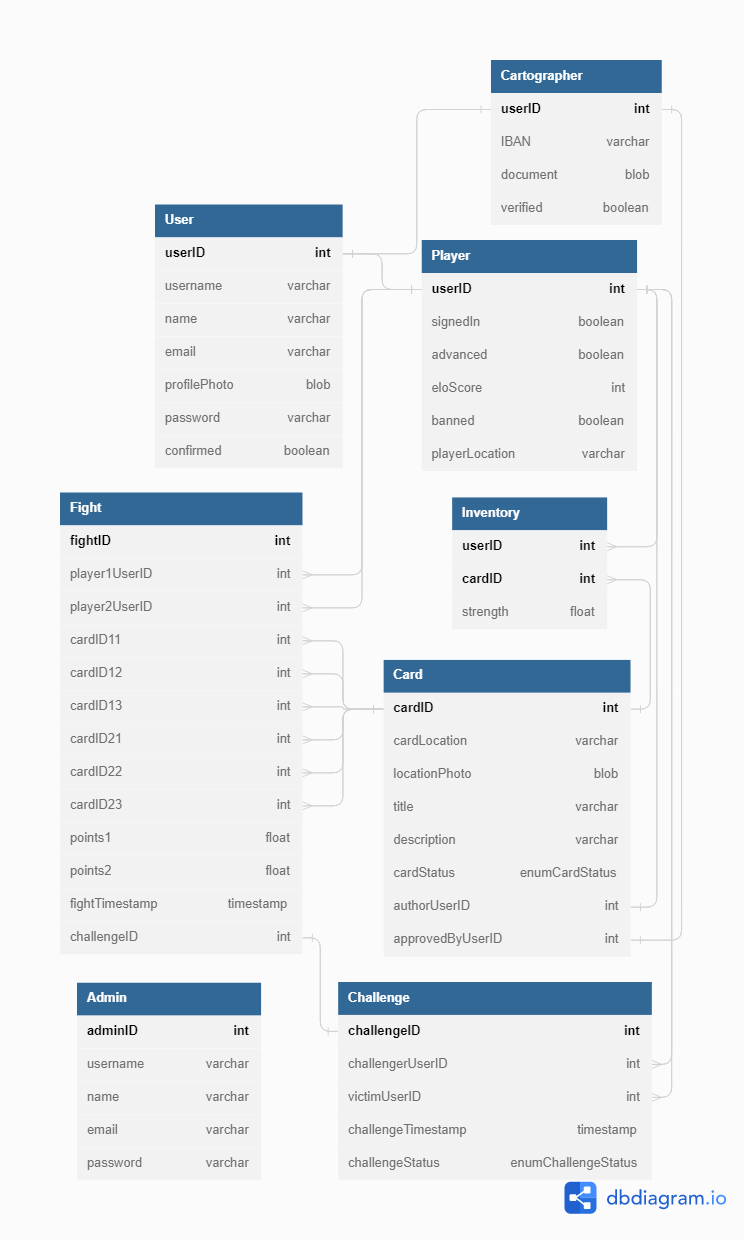
\includegraphics[scale=0.45]{slike/ERdiagram.png}
        			\centering
        			\caption{Dijagram baze podataka}
        			\label{fig:DBmodel}
        		\end{figure}
			
			\eject
			
			
		\section{Dijagram razreda}
		
%	\textit{Potrebno je priložiti dijagram razreda s pripadajućim opisom. Zbog preglednosti je moguće dijagram razlomiti na više njih, ali moraju biti grupirani prema sličnim razinama apstrakcije i srodnim funkcionalnostima.}\\
			
			Slike \ref{fig:classDiagramControllers}, \ref{fig:classDiagramDTO} i \ref{fig:classDiagramModels} prikazuju razrede u \textit{backend} dijelu implementirane MVC arhitekture. S ulogom obrade dolaznih HTTP zahtjeva implementirane su metode u razredima koji nasljeđuju klasu \textit{Controllers}, prikazani na slici \ref{fig:classDiagramControllers}. Pri posluživanju sadržaja i isporuci podataka razredi sa slike \ref{fig:classDiagramControllers} koriste i izmjenjuju \textit{Data transfer objects}, čiji su razredi prikazani na slici \ref{fig:classDiagramDTO}, koje naposlijetku isporučuju u JSON formatu. Za dohvaćanje i implementiranje interakcija među entitetima poput izazova i borbi služe razredi sa slike \ref{fig:classDiagramModels}. 
			\begin{figure}[H]
        			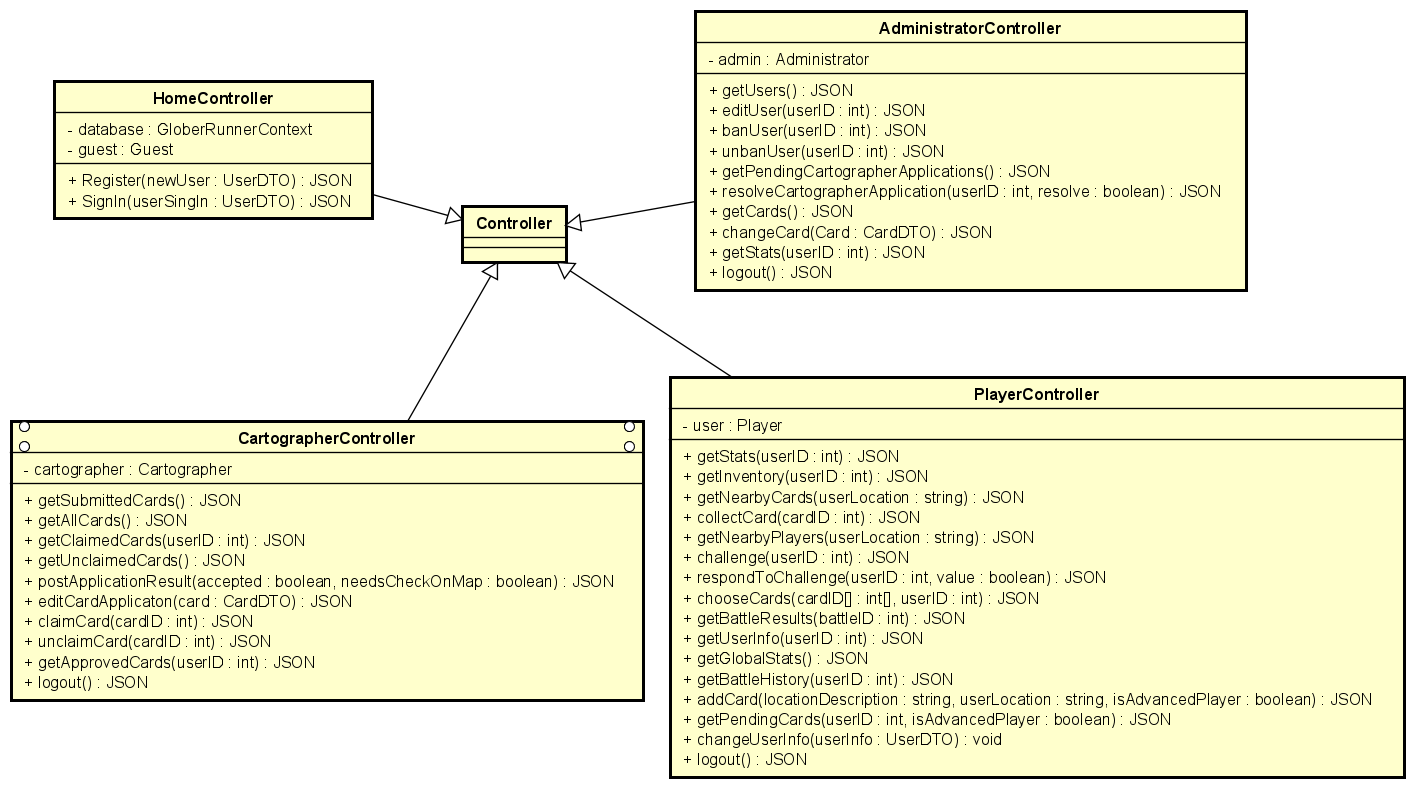
\includegraphics[width=\textwidth]{slike/ClassDiagrams/controllers.png}
        			\centering
        			\caption{Dijagram razreda - dio Controllers}
        			\label{fig:classDiagramControllers}
        		\end{figure}
        		
    		\begin{figure}[H]
    			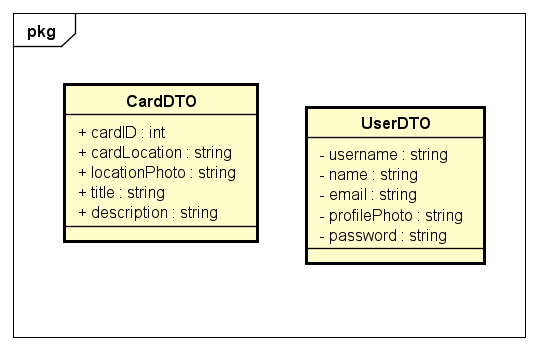
\includegraphics[scale=1]{slike/ClassDiagrams/DTO.png}
    			\centering
    			\caption{Dijagram razreda - dio Data transfer objects}
    			\label{fig:classDiagramDTO}
    		\end{figure}
    		
    		Dijagram koji prikazuje modele sadrži klase koje preslikavaju stvarne entitete u objektnu paradigmu, a uz to omogućuju i komunikaciju s bazom podataka. Razred \textit{Admin} predstavlja administratora koji ima najveće ovlasti i mogućnosti izmjene podataka. \textit{User} je pak apstraktna klasa koja modelira korisnika nastalog registracijom, konkretno to mogu biti \textit{Cartographer} i \textit{Player}, a oni su klase koje nasljeđuju klasu \textit{User} i pružaju specifične funkcionalnosti i komunikaciju s pripadnim relacijama u bazi podataka. Razred \textit{Card} pruža vezu između pripadne relacije u bazi podataka i objektnog modela, a sadrži podatke bitne za prikaz i smještanje kartice u prostoru. Razred \textit{InventoryEntry} povezuje karticu s igračem dodajući joj pritom snagu koja skalira učinak kartice u borbi. Razredom \textit{Challenge} grupiraju se podatci vezani uz izazov koji je jedan igrač uputio drugom, a koji može rezultirati borbom. Klasa \textit{Fight} predstavlja skup podataka koja je potrebna za razrješenje pobjednika neke borbe.
			
			\begin{figure}[H]
        			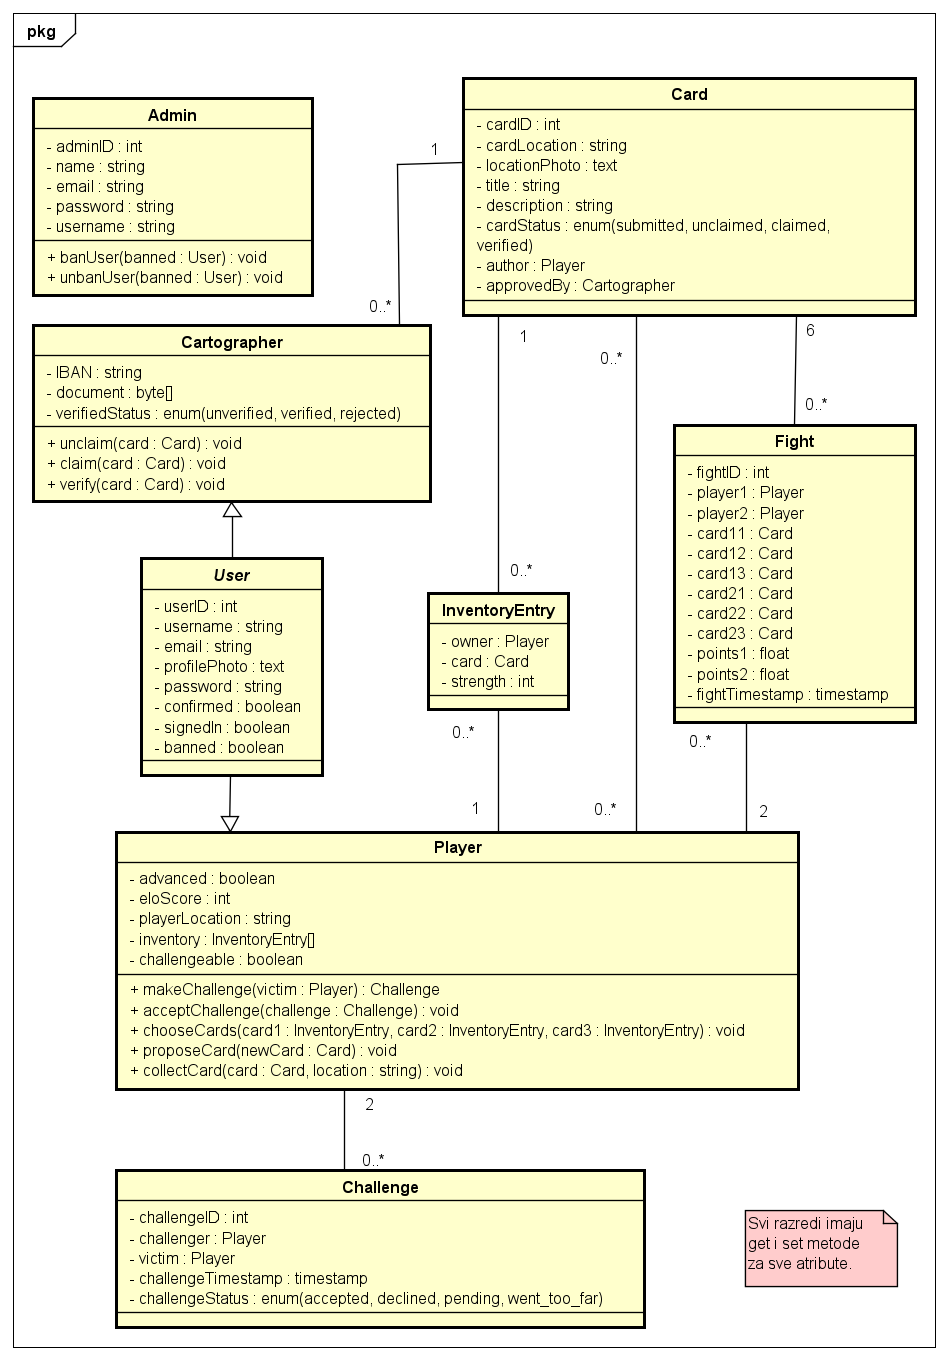
\includegraphics[width=\textwidth]{slike/ClassDiagrams/Models.png}
        			\centering
        			\caption{Dijagram razreda - dio Models}
        			\label{fig:classDiagramModels}
        		\end{figure}
        		
        	
			\iffalse %block com za 1. reviziju
			\textbf{\textit{dio 1. revizije}}\\
			
			\textit{Prilikom prve predaje projekta, potrebno je priložiti potpuno razrađen dijagram razreda vezan uz \textbf{generičku funkcionalnost} sustava. Ostale funkcionalnosti trebaju biti idejno razrađene u dijagramu sa sljedećim komponentama: nazivi razreda, nazivi metoda i vrste pristupa metodama (npr. javni, zaštićeni), nazivi atributa razreda, veze i odnosi između razreda.}\\
			
			\fi %end block com
			
			\pagebreak
			\textbf{\textit{dio 2. revizije}}\\			
			
			\textit{Prilikom druge predaje projekta dijagram razreda i opisi moraju odgovarati stvarnom stanju implementacije}
			
			
			
			\eject
		
		\section{Dijagram stanja}
			
			
			\textbf{\textit{dio 2. revizije}}\\
			
			\textit{Potrebno je priložiti dijagram stanja i opisati ga. Dovoljan je jedan dijagram stanja koji prikazuje \textbf{značajan dio funkcionalnosti} sustava. Na primjer, stanja korisničkog sučelja i tijek korištenja neke ključne funkcionalnosti jesu značajan dio sustava, a registracija i prijava nisu. }
			
			
			\eject 
		
		\section{Dijagram aktivnosti}
			
			\textbf{\textit{dio 2. revizije}}\\
			
			 \textit{Potrebno je priložiti dijagram aktivnosti s pripadajućim opisom. Dijagram aktivnosti treba prikazivati značajan dio sustava.}
			
			\eject
		\section{Dijagram komponenti}
		
			\textbf{\textit{dio 2. revizije}}\\
		
			 \textit{Potrebno je priložiti dijagram komponenti s pripadajućim opisom. Dijagram komponenti treba prikazivati strukturu cijele aplikacije.}